\section{Data Samples}

\subsection{Observed Data
\label{sec:obsdatasamples}}

The observed data analyzed in this dissertation consist of 19.712\fbinv of integrated luminosity, collected by the CMS detector during the 2012 run of the LHC. Figure \ref{fig:lumipublic-dqm} shows the total delivered, recorded, and validated integrated luminosity over time throughout the 2012 run. Events are included in the validated data only if the LHC and the CMS detector were fully operational when the event was recorded. The single electron and single muon primary datasets, listed in Table \ref{tab:data-samples}, are used for the \etau and \mutau channels, respectively. Within the single electron dataset, events are selected if they pass the HLT criterion HLT\_Ele27\_WP80, which requires a reconstructed electron with $\pt>27\GeV$ using the identification working point with 80\% efficiency. Similarly, in the single muon dataset, events are selected if they pass the HLT criterion HLT\_IsoMu24, which requires an isolated reconstructed muon with $\pt>24\GeV$. The average number of interactions per bunch crossing was 21 \cite{LumiPublic}.

\begin{figure}[hbt]
\begin{center}
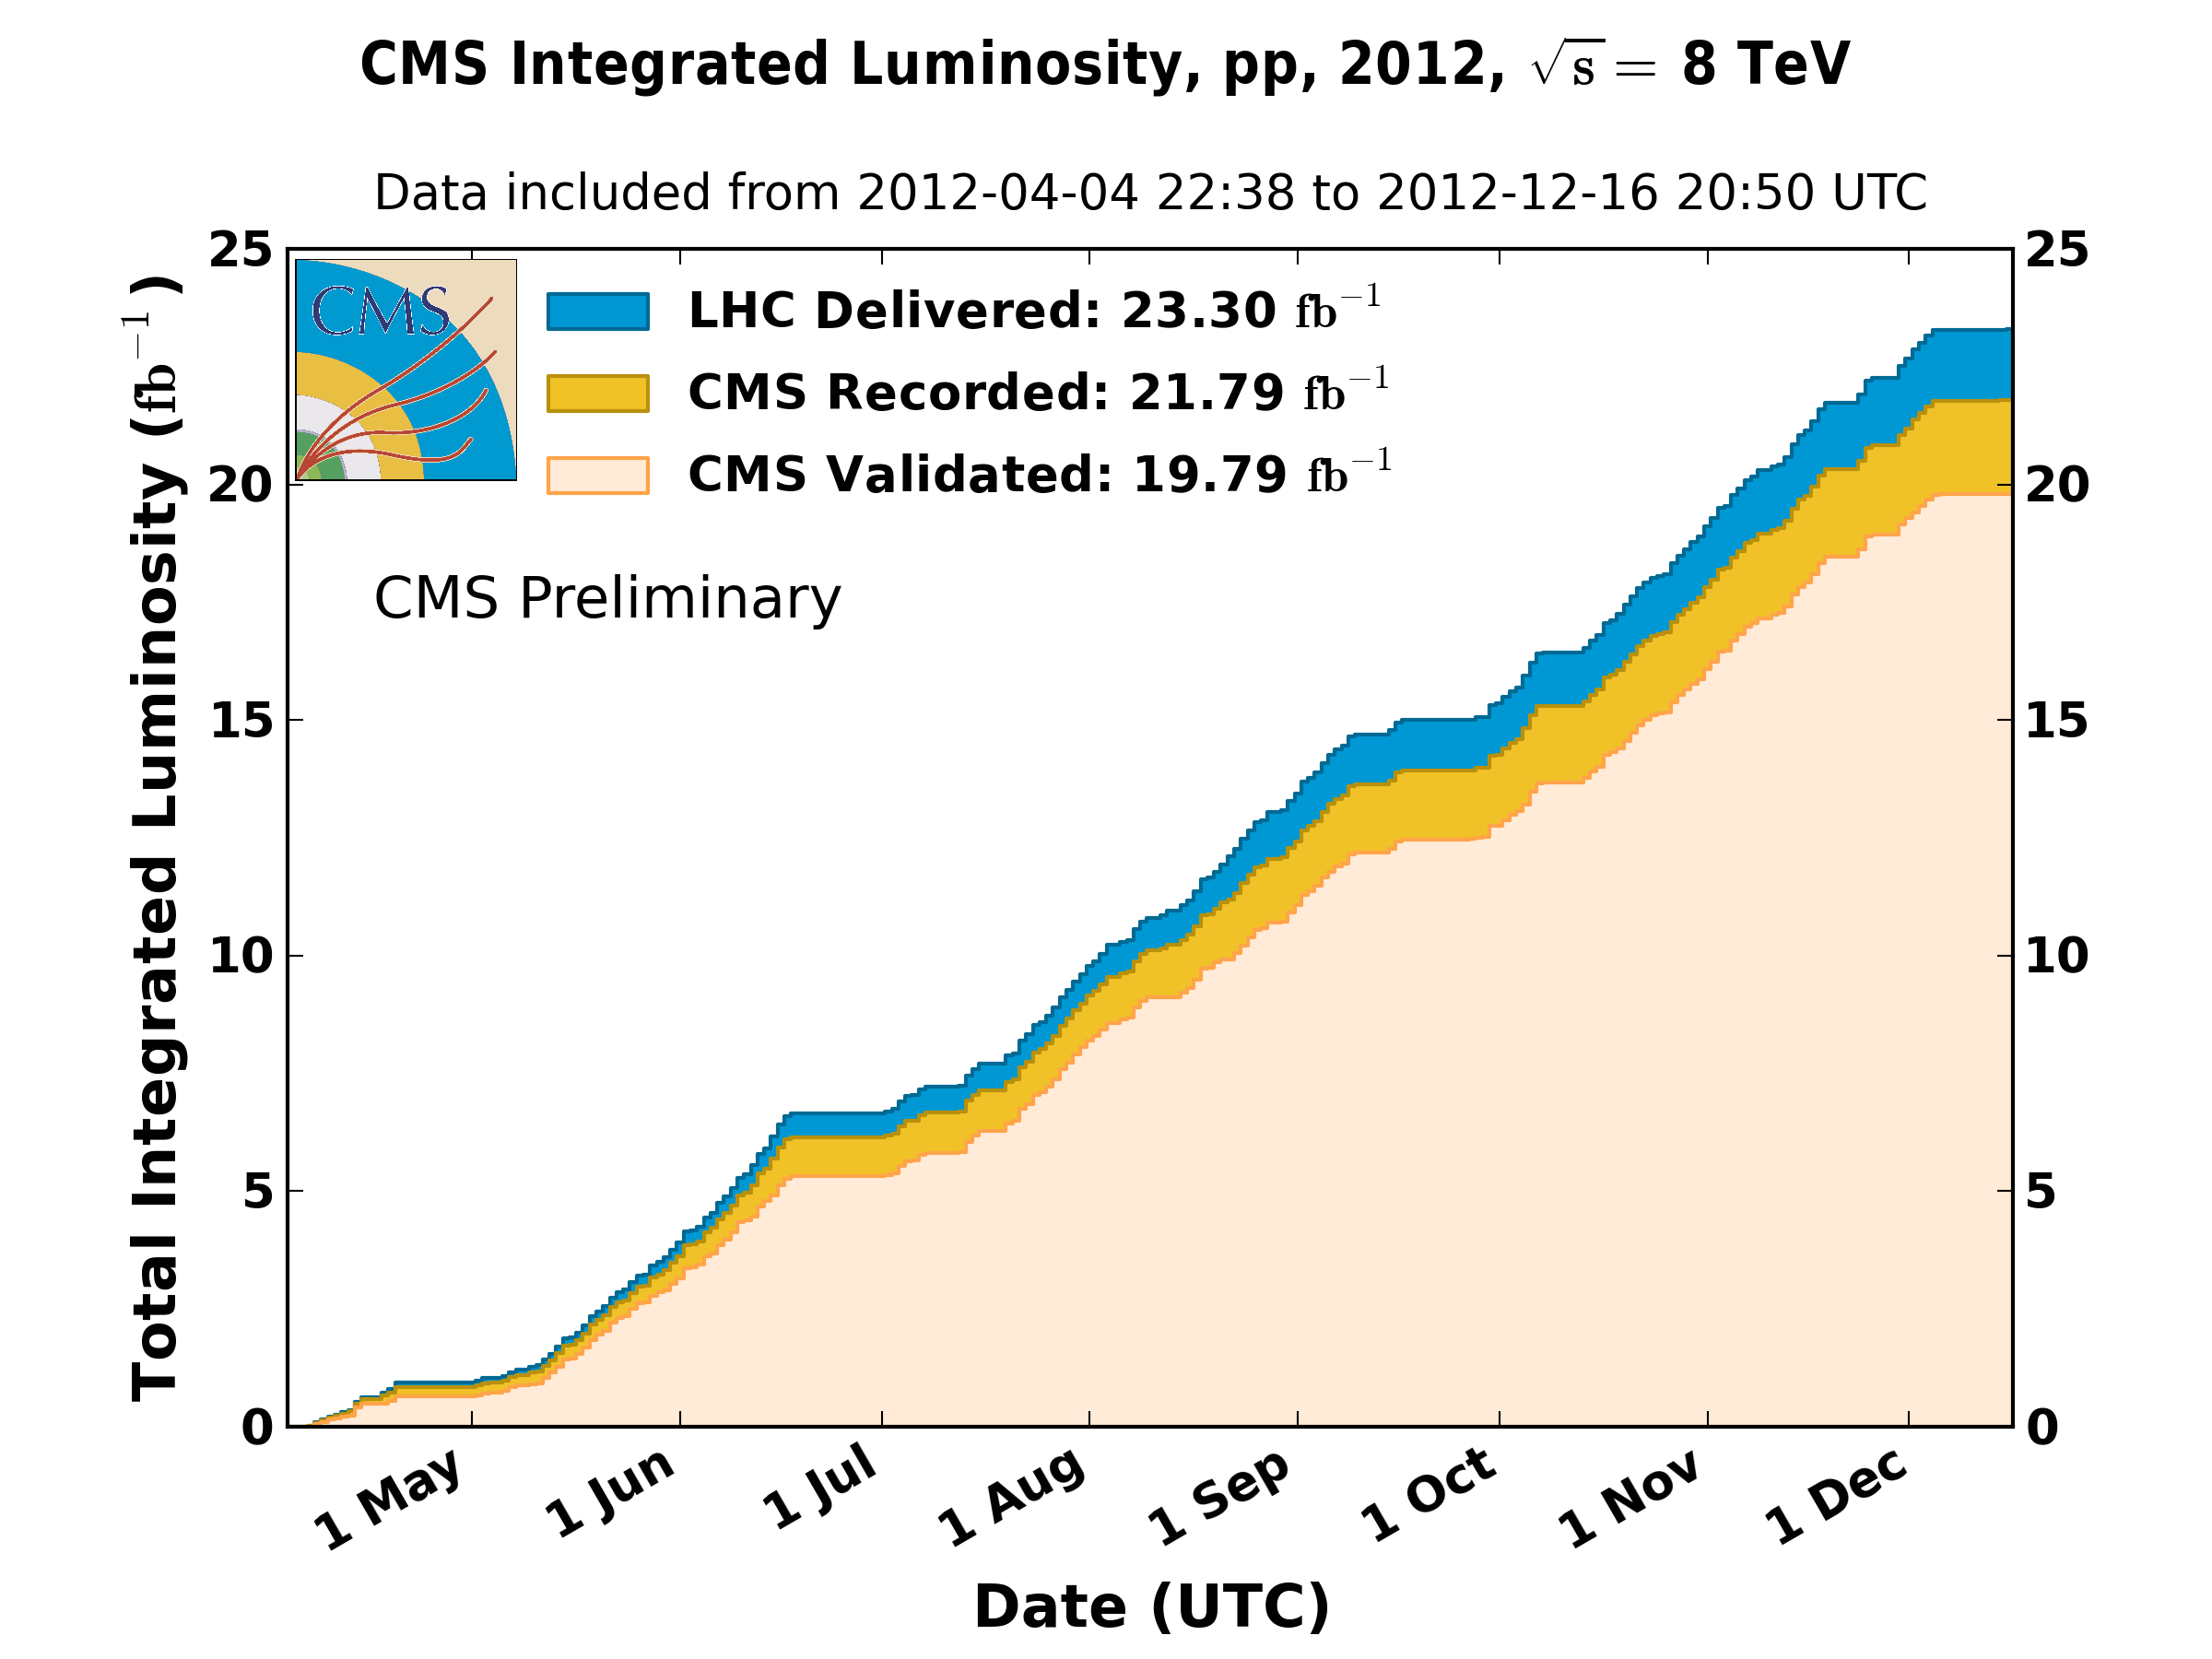
\includegraphics[width=0.95\textwidth]{figures/int_lumi_per_day_cumulative_pp_2012_SummerConf.png}
\caption{A plot of the total integrated luminosity over time for the 2012 run of the LHC, showing the luminosity delivered by the LHC (blue), recorded by the CMS detector (dark orange), and validated as good for physics analysis (light orange) \cite{DataQuality}.}
\label{fig:lumipublic-dqm}
\end{center}
\end{figure}

\begin{table}[hbt]
\begin{center}
\begin{tabular}{|l|}
\multicolumn{1}{c}{$\etau$ channel} \\
\hline
Dataset Name \\
\hline
/SingleElectron/Run2012A-22Jan2013-v1/AOD \\
/SingleElectron/Run2012B-22Jan2013-v1/AOD \\
/SingleElectron/Run2012C-22Jan2013-v1/AOD \\
/SingleElectron/Run2012D-22Jan2013-v1/AOD \\
\hline
\multicolumn{1}{c}{$\mutau$ channel} \\ 
\hline
Dataset Name \\
\hline
/SingleMu/Run2012A-22Jan2013-v1/AOD \\
/SingleMu/Run2012B-22Jan2013-v1/AOD \\
/SingleMu/Run2012C-22Jan2013-v1/AOD \\
/SingleMu/Run2012D-22Jan2013-v1/AOD \\
\hline
\end{tabular}
\caption{The list of observed data samples used in each channel.}
\label{tab:data-samples}
\end{center}
\end{table}

\subsection{Monte Carlo}

Monte Carlo (MC) simulation is used to study the SM background processes which can mimic the signatures of the signal processes. For some processes, the MC simulation is used for the estimation of the final yields and kinematic distributions. For other processes, the final yields and/or kinematic distributions may be estimated from control regions in the observed data. More details on the final background estimations are provided in Sec. \ref{sec:background}. The leptoquark and top squark signal processes are also modeled using MC. A full list of the MC samples used in this dissertation can be found in App. \ref{ch:datasets}.

The \MADGRAPH v5.1.3.30 generator \cite{MadGraph} is used to model the \ttbar, \W+jets, and \Z+jets processes. This generation includes contributions from heavy-flavor and extra jets. For the \ttbar process, an inclusive sample is generated including all decay modes of the two \W bosons from the top quark decays. Exclusive samples with larger numbers of events are also generated, each including only one of three categories for the \W decays: fully leptonic, semileptonic, and fully hadronic. For the \W+jets and \Z+jets processes, inclusive samples including any number of jets are generated. Exclusive samples with larger numbers of events are also generated separately for events with 1 jet, 2 jets, 3 jets, and 4 jets. The single top quark production is modeled with the \POWHEG 1.0 r138 \cite{POWHEG2,POWHEG:singlet,POWHEG:singletW} generator. The \PYTHIA v6.4.24 generator \cite{Sjostrand:2006za} is used to model the diboson processes, including the production of $\W^{+}\W^{-}$, \Wpm\Z, and \Z\Z, collectively denoted as VV. Both the \MADGRAPH and \POWHEG generators are interfaced with \PYTHIA for hadronization and showering. The \TAUOLA program~\cite{TAUOLA} is used for tau lepton decays in all processes which produce genuine tau leptons. The cross sections for the \ttbar and single top quark processes are calculated at next-to-next-to-leading logarithmic (NNLL) accuracy \cite{TOPCrossSec}. The cross sections for the inclusive \W+jets and \Z+jets processes are calculated at NNLO accuracy, while the cross sections for the exclusive production with a specific number of jets are calculated at LO accuracy \cite{FEWZ}. For the VV processes, the cross sections are calculated at NLO accuracy \cite{MCFM}.

The leptoquark and top squark signal processes are generated using \PYTHIA v6.4.24 \cite{Sjostrand:2006za}. The leptoquark pair production process is generated for $\MLQ=200\GeV$ to $\MLQ=1000\GeV$ in steps of 50\GeV, with the decay $\text{LQ} \rightarrow \tau \cPqb$ required. The cross section for leptoquark pair production is calculated at NLO accuracy \cite{LQxsec}. The theoretical uncertainties on these cross sections have been discussed in Sec. \ref{sec:LQ} and are listed in Table \ref{tab:lq-xsec}. As mentioned in Sec. \ref{sec:RPVSUSY}, the deviation between these LQ production cross sections and the corresponding top squark production cross sections is less than 2\%, so the same cross sections can be used to normalize the samples for both signals. The simulation of the chargino-mediated $\lambda_{3jk}^{\prime}$ decay of the top squark is summarized in Table \ref{tab:LQD321-samples}. Samples are generated for $\Mstop=200\GeV$ to $\Mstop=900\GeV$ in steps of 100\GeV. The MSSM parameters for the event generation are $M_1=1000\GeV$, $M_2=1000\GeV$, $M_3=1500\GeV$, $m_{\sLep}=1500\GeV$, $m_{\sQua}=1500\GeV$, $m_{\sNu}=2000\GeV$ and $\text{tan}(\beta)=40$. Here, $M_1$ is the bino mass term, $M_2$ is the wino mass term, and $M_3$ is the gluino mass term. The $\lambda_{321}^{\prime}$ coupling is selected for the generation; because reconstructed light-quark jets are generally indistinguishable regardless of the flavor of the initial quark, these samples can be used to model signals for all $\lambda_{3jk}^{\prime}$ couplings with $j,k=1,2$.

\begin{table}[htb]
  \begin{center}
    \begin{tabular}{|c|c|c|c|c|c|}
\hline
$\Mstop$ $[\GeVns]$    &    $M_{\chipm}$ $[\GeVns]$    &   $\mu$ $[\GeVns]$  & $\lambda_{321}^{\prime}$ & $N_{\text{events}}$ \\
\hline \hline
200   &      100   &  100.98 & 1  &   539,000   \\
300   &      200   &  201.69 & 1  &   50,000   \\
400   &      300   &  302.49 & 1  &   50,000   \\
500   &      400   &  403.46 & 1  &   50,000   \\
600   &      500   &  504.73 & 1  &   50,000   \\
700   &      600   &  606.55 & 1  &   50,000   \\
800   &      700   &  709.47 & 1  &   50,000   \\
900   &      800   &  815.16 & 1  &   50,000   \\
\hline
\end{tabular}
\caption{A summary of the generation of signal samples for the chargino-mediated $\lambda_{3jk}^{\prime}$ decay of the top squark. The chargino mass is determined by the value of $\mu$.}
\label{tab:LQD321-samples}
\end{center}
\end{table}

To account for known discrepancies between the MC simulation and the observed data, various correction factors are applied to the simulated samples. Corrections for the efficiency of muon trigger criteria, identification, and isolation are calculated using tag and probe methods \cite{MuonRefEffs}. Similar correction factors are calculated for electrons \cite{EgammaTagAndProbe,EgammaScaleFactors}. These correction factors depend on the lepton $\pt$ and $\eta$. The chosen working points for the hadronic tau lepton discriminators were found not to need any corrections in the simulation \cite{TauID}. Correction factors for b-tagging and mistagging efficiencies are applied using the method called ``event reweighting using scale factors and MC b-tagging efficiencies'' with the EPS13 prescription \cite{BTagSFMethods}.